\documentclass[a4paper]{article}
\usepackage[spanish]{babel}
\usepackage[utf8]{inputenc}
\usepackage{charter}   % tipografia
\usepackage{graphicx}
%\usepackage{makeidx}

%\usepackage{float}
%\usepackage{amsmath, amsthm, amssymb}
%\usepackage{amsfonts}
%\usepackage{sectsty}
%\usepackage{charter}
%\usepackage{wrapfig}
%\usepackage{listings}
%\lstset{language=C}


\usepackage{color} % para snipets de codigo coloreados
\usepackage{fancybox}  % para el sbox de los snipets de codigo

\definecolor{litegrey}{gray}{0.94}

% \newenvironment{sidebar}{%
% 	\begin{Sbox}\begin{minipage}{.85\textwidth}}%
% 	{\end{minipage}\end{Sbox}%
% 		\begin{center}\setlength{\fboxsep}{6pt}%
% 		\shadowbox{\TheSbox}\end{center}}
% \newenvironment{warning}{%
% 	\begin{Sbox}\begin{minipage}{.85\textwidth}\sffamily\lite\small\RaggedRight}%
% 	{\end{minipage}\end{Sbox}%
% 		\begin{center}\setlength{\fboxsep}{6pt}%
% 		\colorbox{litegrey}{\TheSbox}\end{center}}

\newenvironment{codesnippet}{%
	\begin{Sbox}\begin{minipage}{\textwidth}\sffamily\small}%
	{\end{minipage}\end{Sbox}%
		\begin{center}%
		\colorbox{litegrey}{\TheSbox}\end{center}}



\usepackage{fancyhdr}
\pagestyle{fancy}

%\renewcommand{\chaptermark}[1]{\markboth{#1}{}}
\renewcommand{\sectionmark}[1]{\markright{\thesection\ - #1}}

\fancyhf{}

\fancyhead[LO]{Sección \rightmark} % \thesection\ 
\fancyfoot[LO]{\small{Nombre Apellido, Nombre Apellido, Nombre Apellido}}
\fancyfoot[RO]{\thepage}
\renewcommand{\headrulewidth}{0.5pt}
\renewcommand{\footrulewidth}{0.5pt}
\setlength{\hoffset}{-0.8in}
\setlength{\textwidth}{16cm}
%\setlength{\hoffset}{-1.1cm}
%\setlength{\textwidth}{16cm}
\setlength{\headsep}{0.5cm}
\setlength{\textheight}{25cm}
\setlength{\voffset}{-0.7in}
\setlength{\headwidth}{\textwidth}
\setlength{\headheight}{13.1pt}

\renewcommand{\baselinestretch}{1.1}  % line spacing


% \setcounter{secnumdepth}{2}
\usepackage{underscore}
\usepackage{caratula}
\usepackage{url}


% ******************************************************** %
%              TEMPLATE DE INFORME ORGA2 v0.1              %
% ******************************************************** %
% ******************************************************** %
%                                                          %
% ALGUNOS PAQUETES REQUERIDOS (EN UBUNTU):                 %
% ========================================
%                                                          %
% texlive-latex-base                                       %
% texlive-latex-recommended                                %
% texlive-fonts-recommended                                %
% texlive-latex-extra?                                     %
% texlive-lang-spanish (en ubuntu 13.10)                   %
% ******************************************************** %



\begin{document}


\thispagestyle{empty}
\materia{Organización del Computador II}
\submateria{Primer Cuatrimestre de 2014}
\titulo{Trabajo Práctico II}
\subtitulo{subtitulo del trabajo}
\integrante{Tomas Shaurli}{671/10}{tshaurli@gmail.com}
\integrante{Sebastian Aversa}{379/11}{sebastianaversa@gmail.com}
\integrante{Fernando Gabriel Otero}{424/11}{fergabot@gmail.com}

\maketitle
\newpage

\thispagestyle{empty}
\vfill
\begin{abstract}
En el presente trabajo se describe el an\'alisis de siertos filtros para im\'agenes, comparando las versiones realizadas en C y en assembler con procesamiento SIMD.


El an\'alisis principal ser\'a el tiempo que tardan dichos algoritmos y c\'omo se ha encarado el algoritmo en cada lenguaje.
\end{abstract}
\newpage
\thispagestyle{empty}
\vspace{3cm}
\tableofcontents
\newpage


\normalsize
\newpage

\section{Objetivos generales}

El objetivo de este Trabajo Pr\'actico fue el aprendizaje de las instrucciones SIMD(Single Instruction, Multiple Data) mediante su uso en filtros de im\'agenes, y las comparaciones entre los algoritmos en assembler realizados con \'estas instrucciones y los mismos algoritmos en C.
Tanto en los lenguajes assembler como C se compil\'o y ensambl\'o para arquitecturas Intel x64.



\section{Contexto}

Los algoritmos descriptos y analizados fueron probados en las computadoras de los laboratorios de la facultad. Todas las comparaciones fueron realizadas en las mismas computadoras para un correcto an\'alisis.
Las implementaciones en assembler fueron hechas específicamente para el uso de las instrucciones SIMD de Intel x64 con los siguientes par\'ametros:
\begin{itemize}
	\item -felf64:
	\item -g:
	\item -F:
	\item dwarf:
\end{itemize}
Los sigientes par\'ametros fueron usados en el compilador de C:
\begin{itemize}
	\item ggdb:
	\item -Wall:
	\item -std=c99:
	\item -pedantic:
	\item -m64:
	
	\item pkg-config:
	\item --cflags:
	\item --libs opencv:
\end{itemize}


%\newpage
%\input{introduccion}
\newpage
\section{Filtro de tiles}
\subsection{Enunciado}

 Programar el filtro \textit{tiles} en lenguaje C y luego en ASM haciendo uso de las instrucciones vectoriales (\textbf{SSE}).

\vspace*{0.3cm} \noindent
\textbf{Experimento 1 - análisis el código generado}

Utilizar la herramienta \verb|objdump| para verificar como el compilador de C deja ensamblado el código C. Como es el código generado, ¿cómo se manipulan las variables locales?¿le parece que ese código generado podría optimizarse?

\vspace*{0.3cm} \noindent
\textbf{Experimento 2 - optimizaciones del compilador}

Compile el código de C con optimizaciones del compilador, por ejemplo, pasando el flag \verb|-O1|\footnote{agregando este flag a \texttt{CCFLAGS64} en el makefile}. 
¿Qué optimizaciones realizó el compilador?
¿Qué otros flags de optimización brinda el compilador?
¿Para qué sirven?


\vspace*{0.3cm} \noindent
\textbf{Experimento 3 - secuencial vs. vectorial}

	Realice una medición de las diferencias de performance entre las versiones
	de C y ASM (el primero con -O1, -O2 y -O3).\\
	¿Como realizó la medición?¿Cómo sabe que su medición es una buena medida?¿Cómo afecta a la medición la existencia de \emph{outliers}\footnote{en español, valor atípico: \url{http://es.wikipedia.org/wiki/Valor_atípico}}?¿De qué manera puede minimizar su impacto?¿Qué resultados obtiene si mientras corre los tests ejecuta otras aplicaciones que utilicen al máximo la CPU? 
	Realizar un análisis \textbf{riguroso} de los resultados y acompañar con un gráfico que presente estas diferencias.


\vspace*{0.3cm} \noindent
\textbf{Experimento 4 - cpu vs. bus de memoria}

	Se desea conocer cual es el mayor limitante a la performance de este filtro en su versión ASM.

	¿Cuál es el factor que limita la performance en este caso? En caso de que el limitante
	fuera la intensidad de cómputo, entonces podrían agregarse instrucciones que realicen
	accesos a memoria y la performance casi no debería sufrir. La inversa puede aplicarse
	si el limitante es la cantidad de accesos a memoria.
	
	Realizar un experimento, agregando múltiples instrucciones de un mismo tipo y realizar un análisis
	del resultado. Acompañar con un gráfico.

\vspace*{0.3cm} \noindent
\textbf{Experimento 5 (\textit{opcional}) - secuencial vs. vectorial (parte II)}

	Si vemos a los pixeles como una tira muy larga de bytes, este filtro en
	realidad no requiere ningún procesamiento de datos en paralelo. Esto podría
	significar que la velocidad del filtro de C puede aumentarse hasta casi
	alcanzar la del de ASM. ¿ocurre esto?
	
	Modificar el filtro para que en vez de acceder a los bytes de a uno a la vez
	se accedan como tiras de 64 bits y analizar la performance.
	
\newpage

\subsection{An\'alisis previo}
El filtro de tiles define un rect\'angulo en una imagen en color. La funci\'on debe replicar dicho sector de la im\'agen en el resto de la imagen original.
Para esto, se nos ocurrieron tres formas de encararlo: con la f\'ormula dada en el enunciado (versi\'on C), guardando el primer elemento del rect\'angulo a copiar y guardando un puntero a ese primer elemento.

Formula:

i y j representan fila y columna respectivamente.

dst(i,j) = src [(i mod tamy)+offsety][(j mod tamx)+offsetx]

\subsection{Implementaci\'on en C}

La implementaci\'on en C del ejercicio tiles es tomar un rect\'angulo de la imagen original y repartirla por la imagen destino. Se resuelve con dos ciclos for anidados usando la forma dada en el enuciado.

\subsection{Implementaci\'on en assembler}
Para la resoluci\'on en assembler creamos los dos ciclos anidados con los registros de prop\'osito general. AL comienzo del segundo ciclo se hace la copia.
\begin{codesnippet}
\begin{verbatim}
	MOVDQU XMM0, [RDI]
	MOVDQU [RSI], XMM0
\end{verbatim}
\end{codesnippet}
Luego, para ciclar y recorrer toda la matriz se modifican los valores de RSI y RDI cuando es necesario.
\subsection{Resultado de los experimentos}

\vspace*{0.3cm} \noindent
\textbf{Experimento 1 - análisis el código generado}
\subsubsection{Desensamblado de tiles.o:}
objdump -M intel -d tiles_c.o

tiles_c.o:     formato del fichero elf64-x86-64

Desensamblado de la sección .text:

\begin{codesnippet}
\begin{verbatim}
       push   rbp
       mov    rbp,rsp
       push   r13
       push   r12
       mov    QWORD PTR [rbp-0x58],rdi
       mov    QWORD PTR [rbp-0x60],rsi
       mov    DWORD PTR [rbp-0x64],edx
       mov    DWORD PTR [rbp-0x68],ecx
       mov    DWORD PTR [rbp-0x6c],r8d
       mov    DWORD PTR [rbp-0x70],r9d
       mov    ecx,DWORD PTR [rbp-0x6c]
       movsxd rax,ecx
       sub    rax,0x1
       mov    QWORD PTR [rbp-0x40],rax
       movsxd rax,ecx
       mov    r12,rax
       mov    r13d,0x0
       mov    rax,QWORD PTR [rbp-0x58]
       mov    QWORD PTR [rbp-0x38],rax
       mov    esi,DWORD PTR [rbp-0x70]
       movsxd rax,esi
       sub    rax,0x1
       mov    QWORD PTR [rbp-0x30],rax
       movsxd rax,esi
       mov    r10,rax
       mov    r11d,0x0
       mov    rax,QWORD PTR [rbp-0x60]
       mov    QWORD PTR [rbp-0x28],rax
       mov    DWORD PTR [rbp-0x48],0x0
       jmp    119 <tiles_c+0x119>
 6e    mov    DWORD PTR [rbp-0x44],0x0
       jmp    109 <tiles_c+0x109>
 7a    mov    eax,DWORD PTR [rbp-0x48]
       movsxd rdx,eax
       movsxd rax,esi
       imul   rdx,rax
       mov    rax,QWORD PTR [rbp-0x28]
       lea    rdi,[rdx+rax*1]
       mov    edx,DWORD PTR [rbp-0x44]
       mov    eax,edx
       add    eax,eax
       add    eax,edx
       cdqe   
       add    rax,rdi
       mov    QWORD PTR [rbp-0x20],rax
       mov    eax,DWORD PTR [rbp-0x48]
       cdq    
       idiv   DWORD PTR [rbp+0x18]
       mov    eax,DWORD PTR [rbp+0x28]
       add    eax,edx
       movsxd rdx,eax
       movsxd rax,ecx
       imul   rdx,rax
       mov    rax,QWORD PTR [rbp-0x38]
       lea    r8,[rdx+rax*1]
       mov    edx,DWORD PTR [rbp-0x44]
       mov    eax,edx
       add    eax,eax
       lea    edi,[rax+rdx*1]
       mov    edx,DWORD PTR [rbp+0x10]
\end{verbatim}
\end{codesnippet}
\begin{codesnippet}
\begin{verbatim}
       mov    eax,edx
       add    eax,eax
       lea    r9d,[rax+rdx*1]
       mov    eax,edi
       cdq    
       idiv   r9d
       mov    edi,edx
       mov    edx,DWORD PTR [rbp+0x20]
       mov    eax,edx
       add    eax,eax
       add    eax,edx
       add    eax,edi
       cdqe   
       add    rax,r8
       mov    QWORD PTR [rbp-0x18],rax
       mov    rax,QWORD PTR [rbp-0x20]
       mov    rdx,QWORD PTR [rbp-0x18]
       movzx  edi,WORD PTR [rdx]
       mov    WORD PTR [rax],di
       movzx  edx,BYTE PTR [rdx+0x2]
       mov    BYTE PTR [rax+0x2],dl
       add    DWORD PTR [rbp-0x44],0x1
109    mov    eax,DWORD PTR [rbp-0x44]
       cmp    eax,DWORD PTR [rbp-0x64]
       jl     7a <tiles_c+0x7a>
       add    DWORD PTR [rbp-0x48],0x1
119    mov    eax,DWORD PTR [rbp-0x48]
       cmp    eax,DWORD PTR [rbp-0x68]
       jl     6e <tiles_c+0x6e>
       pop    r12
       pop    r13
       pop    rbp
       ret   
\end{verbatim}
\end{codesnippet}
\begin{codesnippet}
\begin{verbatim}
tiles_asm:
	PUSH RBP	
	MOV RBP, RSP
	XOR R10, R10
	MOV R10D, [RBP+32] ; coloco offsetX
	XOR R11, R11
	.muevoX:
	CMP R11, R10
	JE .bajoY
	LEA RDI, [RDI+3] ;muevo 3 bytes el puntero de la matriz src
	INC R11
	JMP .muevoX
	.bajoY:
	XOR R10, R10
	MOV R10D, [RBP+40] ;coloco offsetY
	XOR R11, R11
	.bajoY2:
	CMP R11, R10
	JE .inicio
	LEA RDI, [RDI+R8] ;aumento en row size bytes el puntero ( bajo una fila)
	INC R11
	JMP .bajoY2
	.inicio:
	MOV R13, RDI
	XOR R11, R11
	XOR R12, R12
	LEA R13, [RDI]
	LEA R12, [RDI]
	XOR R14, R14	; R14: i
	.for1:
		CMP R14, RCX
		JGE .endfor1
		XOR R10, R10
		XOR R15, R15	;R15: j
		MOV RAX, RDI
		.for2:
			CMP R15, RDX
			JGE .endfor2
			CMP R10D, [RBP+16]
			JB .mePaseTile
			XOR R10, R10
			LEA RDI, [R13]
			JMP .for2
			.mePaseTile:
			MOV R11, R10
			ADD R11, 6
			CMP R11D, [RBP+16]
			JBE .sigo
			INC R10
			INC R15
			LEA RDI, [RDI - 13]
			LEA RSI, [RSI - 13]
			MOVDQU XMM0, [RDI]
\end{verbatim}
\end{codesnippet}
\begin{codesnippet}
\begin{verbatim}
			MOVDQU [RSI], XMM0
			LEA RDI, [RDI + 16]
			LEA RSI, [RSI + 16]
			JMP .for2
			.sigo:
			MOV R11, R15
			ADD R11, 6
			CMP R11, RDX
			JBE .sigo2
			INC R10
			INC R15
			;LEA RDI, [RDI - 13]
			LEA RSI, [RSI - 13]
			MOVDQU XMM0, [RDI]
			MOVDQU XMM1, [RSI] ;ME GUARDO LOS ANTERIORES 13 BYTES DE RSI
			PSLLDQ XMM1, 3
			PSRLDQ XMM1, 3
			PSLLDQ XMM0, 13
			PADDB XMM0, XMM1
			MOVDQU [RSI], XMM0s
			LEA RDI, [RDI + 3]
			LEA RSI, [RSI + 16]
			JMP .for2
			.sigo2:
			MOVDQU XMM0, [RDI]
			MOVDQU [RSI], XMM0
			ADD R10, 5
			ADD R15, 5
			LEA RDI, [RDI + 15]
			LEA RSI, [RSI + 15]
			JMP .for2
			.endfor2:
			INC R14
			XOR RAX, RAX
			XOR R15, R15
			MOV EAX, [RBP + 24] ;TAM Y
			MOV R15, R14 ; FILAS QUE RECORRI
			.cicloDiv:
			CMP R15, RAX
			JB .muevoRecuadro
			JE .inicioTiles
			SUB R15, RAX
			CMP R15, RAX
			JG .cicloDiv
			JB .muevoRecuadro
			.inicioTiles:
			LEA RDI, [R12]
			LEA R13, [RDI]
			JMP .muevoDST
			.muevoRecuadro:
			LEA RDI, [R13 + R8]
			LEA R13, [RDI]
\end{verbatim}
\end{codesnippet}
\begin{codesnippet}
\begin{verbatim}
			.muevoDST:
			MOV R15, RDX
			MOV RAX, RDX
			ADD RAX, RAX
			ADD R15, RAX
			MOV RAX, R9
			SUB RAX, R15
			LEA RSI, [RSI + RAX]
			JMP .for1
	.endfor1:
	POP RBP
	RET
\end{verbatim}
\end{codesnippet}


\vspace*{0.3cm} \noindent
\textbf{Experimento 2 - optimizaciones del compilador}
El compilador ofrece los flags -O1 a -03 para distintos niveles de optimizaci\'on, asi como los flags para indicar si es assembler de intel, amd, etc. 
Esto ultimo hace m\'as espec\'ifico el codigo assembler y correr\'ia mejor en una maquina con el microprocesador seleccionado,aunque no correr\'ia en uno de otra marca o de una familia de microprocesadores anterior a la elegida.

\vspace*{0.3cm} \noindent
\textbf{Experimento 3 - secuencial vs. vectorial}

\vspace*{0.3cm} \noindent
\textbf{Experimento 4 - cpu vs. bus de memoria}

\vspace*{0.3cm} \noindent
\textbf{Experimento 5 (\textit{opcional}) - secuencial vs. vectorial (parte II)}

\newpage
\section{Filtro Popart}
\subsection{Enunciado}

\subsection*{Filtro \textit{Popart}}

  Programar el filtro \textit{Popart} en lenguaje C y en en ASM haciendo uso de 
  las instrucciones vectoriales (\textbf{SSE}).

\vspace*{0.3cm} \noindent
\textbf{Experimento 1 - saltos condicionales}

	Se desea conocer que tanto impactan los saltos condicionales
	en el código del ejercicio anterior con \verb|-O1|.\\
	Para poder medir esto, una posibilidad es quitar las comparaciones
	al procesar cada pixel. Por más que la imagen resultante no sea correcta,
	será posible tomar una medida del impacto de los saltos condicionales.
	Analizar como varía la performance. 
	
	Si se le ocurren, mencionar otras posibles formas de medir el impacto de los saltos condicionales.

\vspace*{0.3cm} \noindent
\textbf{Experimento 2 - cpu vs. bus de memoria}

	¿Cuál es el factor que limita la performance en este caso? 
	
	Realizar un experimento, agregando múltiples instrucciones de un mismo tipo
	y realizar un análisis 	del resultado. Acompañar con un gráfico.


\vspace*{0.3cm} \noindent
\textbf{Experimento 3 - prefetch}

  La técnica de \textit{prefetch} es otra forma de optimización que puede
  realizarse. Su sustento teórico es el siguiente:
  
  Suponga un algoritmo que en cada iteración tarda n ciclos en obtener un dato y una cantidad
  similar en procesarlo. Si el algoritmo lee el dato $i$ y luego lo procesa,
  desperdiciará siempre n ciclos esperando entre que el dato llega y que se comienza
  a procesar efectivamente. Un algoritmo más inteligente podría pedir el 
  dato $i+1$ al comienzo del ciclo de proceso del dato $i$ (siempre suponiendo
  que el dato $i$ pidió en la iteración $i-1$. De esta manera, a la vez que el
  procesador computa todas las instrucciones de la iteración $i$, se estáran trayendo
  los datos de la siguiente iteración, y cuando esta última comience, los datos ya
  habrán llegado.

  \vspace*{0.2cm}
  Estudiar esta técnica y proponer una aplicación al código del filtro en la versión ASM.
  Programarla y analizar el resultado. ¿Vale la pena hacer prefetching?

\vspace*{0.3cm} \noindent
\textbf{Experimento 3 - secuencial vs. vectorial}

  Analizar cuales son las diferencias de performace entre las versiones de C y ASM. 
  Realizar gráficos que representen estas diferencias.


\subsection{An\'alisis previo}
El algoritmo de popart reemplaza cada pixel por uno de cinco pixeles preseleccionados. 
La elecci\'on resulta de la suma de los elementos del pixel.

En un primer an\'alisis, el filtro popart tiene 3 partes: el ciclo, la suma de los elementos rgb, y la elecci\'on del pixel de reemplazo.

\subsection{Implementaci\'on en C}
Para la implementaci\'on en C usamos un vector con los posibles reemplazos para cada pixel, 
y una funci\'on que devuelve cual va a ser ese reemplazo mediante comparaciones.
\begin{codesnippet}
\begin{verbatim}

rgb_t colores[] = { {255,   0,   0},
                    {127,   0, 127},
                    {255,   0, 255},
                    {  0,   0, 255},
                    {  0, 255, 255} };

			
int pop_art(unsigned int r, unsigned int g, unsigned int b)
{
    unsigned int suma = r + g + b;
    int res;
	
    if 		 (suma < 153)	{res = 0;}
    else if (suma < 306)	{res = 1;}
    else if (suma < 459)	{res = 2;}
    else if (suma < 612)	{res = 3;}
    else 					{res = 4;}
	
    return res;
}
\end{verbatim}
\end{codesnippet}

\subsection{Implementaci\'on en assembler}
Armamos máscaras para las comparaci\'ones con suma(i,j).
\begin{codesnippet}
\begin{verbatim}
seisDoce:          DD 0x264, 0x264, 0x264, 0x264    ; 612, 612, 612, 612			
cuatroCincoNueve:  DD 0x1CB, 0x1CB, 0x1CB, 0x1CB    ; 459, 459, 459, 459	
tresOSeis:         DD 0x132, 0x132, 0x132, 0x132    ; 306, 306, 306, 306	
unoCincoTres:      DD 0x99, 0x99, 0x99, 0x99        ; 153, 153, 153, 153
\end{verbatim}
\end{codesnippet}

Tambi\'en para reemplazar los pixeles (solo cito el primer caso).
\begin{codesnippet}
\begin{verbatim}
colores0:          DB  0xFF, 0x0,  0x0, 0x0,        ; 255,   0,   0,   0
                   DB  0xFF, 0x0,  0x0, 0x0,        ; 255,   0,   0,   0
                   DB  0xFF, 0x0,  0x0, 0x0,        ; 255,   0,   0,   0
                   DB  0xFF, 0x0,  0x0, 0x0         ; 255,   0,   0,   0

\end{verbatim}
\end{codesnippet}
El resto de las m\'ascaras, usadas con \verb|PSHUFB|.\\ son:

\begin{itemize}
	\item pixel0BGR : Para tener un pixel (R,G y B) en cada \textit{double word}. El cuarto Byte se rellena con ceros
			
	\item soloPrimero : Lo usamos para trabajar sobre el primer Byte de cada \textit{double word}
		
	\item pixelFinal : Sirve para sacar el ceros ubicado en el cuarto Byte de cada \textit{double word}. El ultimo DB se rellena con ceros
\end{itemize}
\'Estas m\'ascaras son usadas en \textit{pop_art} para discriminar los Bytes de R, G y B y guardar la suma de cada uno en un \textit{double word}

El uso de \textit{double word} viene del hecho de que un pixel se compone de tres elementos de un Byte cada uno, 
y necesitamos tener cada pixel en una cantidad par de Bytes para poder desempaquetar correctamente. Esto nos lleva a usar 4 Bytes por cada pixel.

Otra parte del codigo importante es el que genera la sumatoria, para lo cual utilizamos los \verb|PSHUFB|:\\
\begin{codesnippet}
\begin{verbatim}
	MOVDQU XMM0, [RDI]	; R|G|B|R|G|B|R|G|B|R|G|B|R|G|B|R coloco los primeros 16bytes 
                        ; de la imagen en XMM1

    XORPD XMM2, XMM2
    XORPD XMM3, XMM3
    XORPD XMM4, XMM4
    MOVDQA XMM7, [pixel0BGR]
    PSHUFB XMM0, XMM7              ; ordeno en el registro los pixels de forma 0RGB 
                                   ; (tengo 4 pixeles)
    MOVDQU XMM2, XMM0              ; XMM2: R|G|B|0|R|G|B|0|R|G|B|0|R|G|B|0
    PSHUFB XMM2, [soloPrimero]     ; XMM2: R|0|0|0|R|0|0|0|R|0|0|0|R|0|0|0
                                   ; solo dejamos azul para 'suma'
    MOVDQU XMM3, XMM0              ; XMM3: R|G|B|0|R|G|B|0|R|G|B|0|R|G|B|0 	
    PSRLD XMM3, 8                  ; XMM3: G|B|0|0|G|B|0|0|G|B|0|0|G|B|0|0		
    PSHUFB XMM3, [soloPrimero]     ; XMM3: G|0|0|0|G|0|0|0|G|0|0|0|G|0|0|0
                                   ; solo dejamos verde para 'suma'
    MOVDQU XMM4, XMM0              ; XMM4: R|G|B|0|R|G|B|0|R|G|B|0|R|G|B|0 	
    PSRLD XMM4, 16                 ; XMM4: B|0|0|0|B|0|0|0|B|0|0|0|B|0|0|0
                                   ; solo dejamos rojo para 'suma'
    ;Ahora podemos hacer suma
    PADDW XMM2, XMM3
    PADDW XMM2, XMM4               ; XMM2: dword[R+G+B] dword[R+G+B] dword[R+G+B] dword[R+G+B]
\end{verbatim}
\end{codesnippet}

\subsection{Resultado de los experimentos}
%\begin{figure}
%  \begin{center}
%	
\includegraphics[scale=0.66]{imagenes/logouba.jpg}
%	\caption{Logo}
%	\label{Logo}
%  \end{center}
%\end{figure}
\vspace*{0.3cm} \noindent
\textbf{Experimento 1 - saltos condicionales}

\vspace*{0.3cm} \noindent
\textbf{Experimento 2 - cpu vs. bus de memoria}

\vspace*{0.3cm} \noindent
\textbf{Experimento 3 - prefetch}

\vspace*{0.3cm} \noindent
\textbf{Experimento 3 - secuencial vs. vectorial}

\newpage
\section{Filtro Temperature}
\subsection{Enunciado}

\subsection*{Filtro \textit{Temperature}}

  Programar el filtro \textit{Temperature} en lenguaje C y en en ASM haciendo uso de 
  las instrucciones vectoriales (\textbf{SSE}).


\vspace*{0.3cm} \noindent
\textbf{Experimento 1}

  Analizar cuales son las diferencias de performace entre las versiones de C y ASM. 
  Realizar gráficos que representen estas diferencias.
  
\subsection{An\'alisis previo}

El filtro temperature nuevamente presenta tres partes: el ciclo, la elecci\'on de c\'omo modificar los pixeles y la modificaci\'on propiamente dicha.

En \'este caso, la eleccin de los pixeles sale del promedio de los elementos RGB, y la modificaci\'on se realiza en base al promedio.

\subsection{Implementaci\'on en C}

En este caso no separamos la comparacion del pixel de su modificaci\'on porque cada pixel se modifica usando el valor del promedio de los valores RGB. El resto de la implementaci\'on es el ciclo del main que recorre toda la imagen.

\begin{codesnippet}
\begin{verbatim}
void temperatura(rgb_t* p_d, unsigned int r, unsigned int g, unsigned int b)
{
    unsigned int prom = (r + g + b) / 3;

    if 		(prom < 32)		{p_d->r = 0; 				p_d->g = 0; 				p_d->b = 128 + 4*prom;}
    else if (prom < 96)		{p_d->r = 0; 				p_d->g = -128 + 4*prom; 	p_d->b = 255;}
    else if (prom < 160)	{p_d->r = -384 + 4*prom;	p_d->g = 255; 				p_d->b = 639 - 4*prom;}
    else if (prom < 224)	{p_d->r = 255; 				p_d->g = 895 - 4*prom;	 	p_d->b = 0;}
    else 					{p_d->r = 1151 - 4*prom;	p_d->g = 0; 				p_d->b = 0;}
}
\end{verbatim}
\end{codesnippet}
\subsection{Implementaci\'on en assembler}

En este algoritmo tenemos ciertas partes muy parecidas a \textit{popart_asm}, como la sumatoria de los elementos RGB con \verb|PSHUFB| 
(para luego dividir por tres y obtener el promedio).

Sin embargo en este caso estas partes fueron encaradas de forma distinta. \\
Si comparamos los 2 algoritmos que realizan \verb|PSHUFB|, el algoritmo de la funci\'on \textit{popart} trabaja de a 4 pixels y la funci\'on 
\textit{temp_aux} de a 2 pixels.

Pero por ciclo, \textit{temperature_asm} procesa 5 pixeles en vez de los 4 que procesa \textit{popart_asm} por ciclo
\subsubsection{tempe:}
\begin{codesnippet}
\begin{verbatim}
tempe:
    PUSH RBP
    MOV RBP, RSP
        ;XMM0: R|G|B|R|G|B|R|G|B|R|G|B|R|G|B|R coloco los primeros 16bytes de la imagen en XMM1
        ;XMM0: 0|1|2|3|4|5|6|7|8|9|10|11|12|13|14|15
        ;llamare al resultado: R0|R1|R2|R3|R4|R5|R6|R7|R8|R9|R10|R11|R12|R13|R14|-
        MOVDQU XMM8, XMM0
        CALL temp_aux
        MOVDQU XMM9, XMM0
        PSHUFB XMM8, [moverPixeles]  ; XMM8: 6 |7 |8 |9 |10|11|12|13|14|15|- |- |- |- |- |-
        PSHUFB XMM9, [moverPixeles2] ; XMM9: - |- |- |- |- |- |- |- |- |R0|R1|R2|R3|R4|R5|-
        MOVDQU XMM0, XMM8	
        CALL temp_aux
        MOVDQA XMM13, XMM0
        PSHUFB XMM13, [moverPixeles3]; xmm13: - |- |- |R6|R7|R8|R9|R10|R11|- |- |- |- | -|- |-

        PSHUFB XMM8, [moverPixeles1] ; xmm8:  12|13|14|- |- |- |- |- |- |- |- |- |- |- |- |-
        MOVDQU XMM0, XMM8
        CALL temp_aux                ; xmm0:  R12|R13|R14|basura
        PSHUFB XMM0, [unPixel]       ; xmm0:  R12|R13|R14|- |- |- |- |- |- |- |- |- |- |- |- |-

        POR XMM0, XMM13              ; xmm0: R12|R13|R14|R6|R7|R8|R9|R10|R11|- |- |- |- |- |- |-
        POR XMM0, XMM9               ; xmm0: R12|R13|R14|R6|R7|R8|R9|R10|R11|R0|R1|R2|R3|R4|R5|-
        PSHUFB XMM0, [invertir]      ; xmm0: R0|R1|R2|R3|R4|R5|R6|R7|R8|R9|R10|R11|R12|R13|R14|-
    POP RBP
    RET
\end{verbatim}
\end{codesnippet}

\subsubsection{temp_aux:}

En la primer parte de \'esta funci\'on auxiliar usamos m\'ascaras para separar los colores y sumarlos entre si, dos pixeles al mismo tiempo.
Luego armamos para dividir este valor por tres, dando el promedio.
\begin{codesnippet}
\begin{verbatim}
temp_aux:
    
    PUSH RBP					
    MOV RBP, RSP
    PUSH R12
    PUSH R13
    
    
    XORPD XMM2, XMM2
    XORPD XMM3, XMM3
    XORPD XMM4, XMM4
    
    MOVDQA XMM7, [pixel0BGR]
    PSHUFB XMM0, XMM7		 			; ordeno en el registro los pixels de forma 0RGB (tengo 4 pixeles)
    MOVDQU XMM2, XMM0					; XMM2: R|0|G|0|B|0|0|0|R|0|G|0|B|0|0|0	
    PSHUFB XMM2, [soloPrimero]			; XMM2: R|0|0|0|0|0|0|0|R|0|0|0|0|0|0|0
    MOVDQU XMM3, XMM0					; XMM3: R|0|G|0|B|0|0|0|R|0|G|0|B|0|0|0 	
    PSRLQ XMM3, 16						; XMM3: G|0|B|0|0|0|0|0|G|0|B|0|0|0|0|0		
    PSHUFB XMM3, [soloPrimero]			; XMM3: G|0|0|0|0|0|0|0|G|0|0|0|0|0|0|0
    MOVDQU XMM4, XMM0					; XMM4: R|0|G|0|B|0|0|0|R|0|G|0|B|0|0|0 	
    PSRLQ XMM4, 32						; XMM4: B|0|0|0|0|0|0|0|B|0|0|0|0|0|0|0
        ; Ahora podemos hacer suma
    PADDQ XMM2, XMM3
    PADDQ XMM2, XMM4					; XMM2: qword[R+G+B] qword[R+G+B] 
    
    XORPD XMM5, XMM5
    ;///////////////////////////////////////////////////////////////////////////////////////////////////
        ; suma / 3
    MOV R12, 3
    MOV R13, 1
    XORPD XMM0, XMM0
    XORPD XMM1, XMM1
    CVTSI2SS XMM0, R12
    CVTSI2SS XMM1, R13
        ; PARA EXTENDER EL 3 A LOS PACKS DEL XMM5
    XORPD XMM5, XMM5
    ADDSS XMM5, XMM1
    PSLLDQ XMM5, 4
    ADDSS XMM5, XMM0
    PSLLDQ XMM5, 4
    ADDSS XMM5, XMM1
    PSLLDQ XMM5, 4
    ADDSS XMM5, XMM0
    
    CVTDQ2PS XMM2, XMM2
    DIVPS XMM2, XMM5					; XMM2: prom (float)
    CVTTPS2DQ XMM2, XMM2
    CVTDQ2PS XMM2, XMM2
    MOVDQU XMM12, XMM2					; XMM12: prom (float)
    CVTTPS2DQ XMM12, XMM12
        ;XMM2: [T|0|0|0|0|0|0|0] [T|0|0|0|0|0|0|0]
\end{verbatim}
\end{codesnippet}

En esta segunda parte se elije mediante m\'ascaras qu\'e pixel ser\'a devuelto. 
\begin{codesnippet}
\begin{verbatim}
    XORPD XMM0, XMM0
        ; ponemos colores[0] en su lugar correspondiente	{128 + 4t, 0, 0}
    
    MOVDQU XMM10, [colores0] 			; XMM10: qword[128(+4T)] qword[128(+4T)] 
    
        ;XMM10: colores[0] nos falta agregar 4T
        ;XMM2: [T|0|0|0|0|0|0|0] [T|0|0|0|0|0|0|0]
    MOVDQU XMM6, XMM2
        ;XMM6: [T|0|0|0|0|0|0|0] [T|0|0|0|0|0|0|0]
    
        ;PARA MULTIPLICAR POR 4
    MOV R12, 4
    XORPD XMM14, XMM14
    MOVQ XMM14, R12
    XORPD XMM5, XMM5
    PADDQ XMM5, XMM14
    PSLLDQ XMM5, 8
    PADDQ XMM5, XMM14
    
    CVTDQ2PS XMM5, XMM5
    MULPS XMM6, XMM5	; XMM6: qword[4T|0|0|0|0|0|0|0] qword[4T|0|0|0|0|0|0|0]
    
    CVTTPS2DQ XMM6, XMM6
    
        ; A: 4T + 128
        ; XMM6: 	qword[4T|0|0|0|0|0|0|0] 		qword[4T|0|0|0|0|0|0|0]
        ; XMM10: 	qword[128(+4T)|0|0|0|0|0|0|0] 	qword[128(+4T)|0|0|0|0|0|0|0]
    PADDUSW XMM10, XMM6
    MOVDQU XMM6, XMM10
        ;XMM10 == XMM6 == qword[4T+128] qword[4T+128]
    XORPD XMM15, XMM15
    PUNPCKLQDQ XMM10, XMM15
    PUNPCKHQDQ XMM6, XMM15
        ;XMM10 == qword{[A|0|0|0|0|0|0|0] [0|0|0|0|0|0|0|0]}
        ;XMM6 ==  qword{[A|0|0|0|0|0|0|0] [0|0|0|0|0|0|0|0]}
        ;Lo voy a mirar de otra forma para empaquetar (puedo porque con 16bits me alcanza para representar A):
        ;XMM10 == dword{[A|0] [G|0] [B|0] [0|0] [0|0] [0|0] [0|0] [0|0]}
        ;XMM6 ==  dword{[A|0] [G|0] [B|0] [0|0] [0|0] [0|0] [0|0] [0|0]}
    PACKUSWB XMM10, XMM6
        ;XMM10 == dword{[AGB0][0000][AGB0][0000]}
        ;empaquete saturando word a byte para reducir el tamanio de A de 2 bytes a 1 byte
    PSHUFB XMM10, [shuffleCaverna2]
        ;XMM10 == dword{[AGB0][AGB0][0000][0000]}
    
    MOVDQU XMM1, [tresDos] 
    PCMPGTD XMM1, XMM12	
    PSHUFB XMM1, [shuffleCaverna2]
    PAND XMM1 , XMM10 					; estos pixeles le ponemos colores[0]
    XORPD XMM0, XMM0
    POR XMM0, XMM1						; ponemos colores0 en donde va en dst
	;///////////////////////////////////////////////////////////////////////////////////////////////////

        ; ponemos colores[4] en su lugar correspondiente	{  0, 0, 1151 -4t}

        ;Codigo no copiado. Se repite el proceso que con [colores0]
	;///////////////////////////////////////////////////////////////////////////////////////////////////

        ; ponemos colores[3] en su lugar correspondiente     {0, 895 - 4t, 255}

        ;Codigo no copiado. Se repite el proceso que con [colores0]
	;///////////////////////////////////////////////////////////////////////////////////////////////////

        ; ponemos colores[2] en su lugar correspondiente		{639 -4t, 255, -384 + 4t},	

        ;Codigo no copiado. Se repite el proceso que con [colores0]
    ;///////////////////////////////////////////////////////////////////////////////////////////////////

        ; ponemos colores[1] en su lugar correspondiente		{255, -128 + 4t, 0}

        ;Codigo no copiado. Se repite el proceso que con [colores0]
    ;///////////////////////////////////////////////////////////////////////////////////////////////////	
    
    
        ;ahora en XMM2 tenemos dst con los colores finales
        ;sacamos los ceros para que queden pixeles de 3 bytes
        
        
    MOVDQU XMM10, [pixelFinal] ; [ 0 , 1 , 2 , 4, 5 , 6 , - , -, - , - , - , -, - , - , - , -]
    PSHUFB XMM0, XMM10
    
    POP R13
    POP R12
    POP RBP
    RET
\end{verbatim}
\end{codesnippet}

\subsection{Resultado de los experimentos}
\vspace*{0.3cm} \noindent
\textbf{Experimento 1}


%\paragraph{\textbf{Titulo del parrafo} } Bla bla bla bla.
%Esto se muestra en la figura~\ref{nombreparareferenciar}.

%\begin{codesnippet}
%\begin{verbatim}

%struct Pepe {
%
%    ...
%
%};
%\end{verbatim}
%\end{codesnippet}

%\begin{figure}
%  \begin{center}
%	
\includegraphics[scale=0.66]{imagenes/logouba.jpg}
%	\caption{Logo}
%	\label{Logo}
%  \end{center}
%\end{figure}



\newpage
\section{Filtro LDR}
\subsection{Enunciado}

\subsection*{Filtro \textit{LDR}}
  Programar el filtro \textit{LDR} en lenguaje C y en
  ASM haciendo uso de las instrucciones \textbf{SSE}.

\vspace*{0.3cm} \noindent
\textbf{Experimento 1}

  Analizar cuales son las diferencias de performace entre las versiones de C y ASM. 
  Realizar gráficos que representen estas diferencias.
  
\subsection{An\'alisis previo}

\subsection{Implementaci\'on en C}
\paragraph{\textbf{Titulo del parrafo} } Bla bla bla bla.
Esto se muestra en la figura~\ref{nombreparareferenciar}.
\subsection{Implementaci\'on en assembler}
\begin{codesnippet}
\begin{verbatim}

struct Pepe {

    ...

};
\end{verbatim}
\end{codesnippet}
\subsection{Resultado de los experimentos}

\vspace*{0.3cm} \noindent
\textbf{Experimento 1}

\begin{figure}
  \begin{center}
	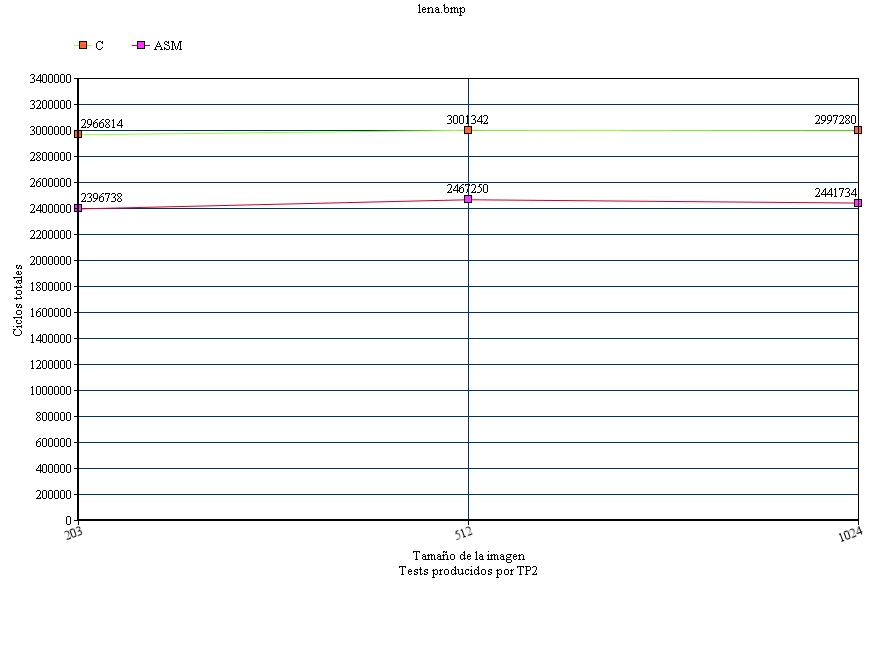
\includegraphics[scale=0.66]{imagenes/ldr-lena.jpg}
	\caption{Lena}
	\label{Lena}
  \end{center}
\end{figure}

\begin{figure}
  \begin{center}
	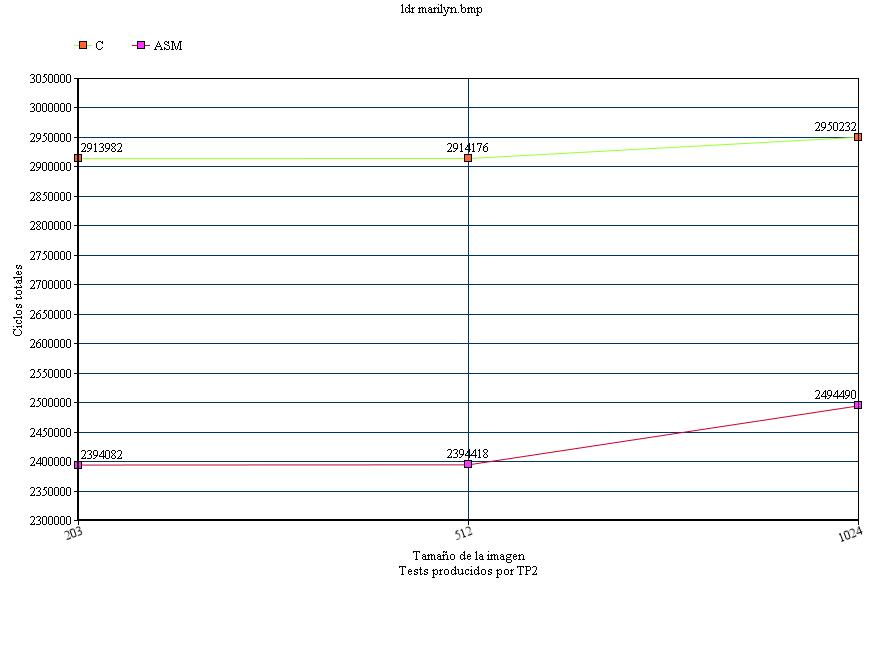
\includegraphics[scale=0.66]{imagenes/ldr-marilyn.jpg}
	\caption{Marilyn}
	\label{Marilyn}
  \end{center}
\end{figure}

Realizamos los tests armando un ciclo de 100000 ejecuciones del mismo c\'odigo con las mismas entradas, y a su vez ejecutamos estos tests 5 veces para cada entrada. \'Esto nos 
permiti\'o hacer promedios y descartar tests que daban muy lejos del valor medio.

Como muestran los gr\'aficos presentados, hay claras diferencias de velocidad (medida en cantidad de ciclos) entre uno y otro lenguaje. Tambi\'en notamos que no hay una gran 
variaci\'on de velocidad entre los distintos tamaños de las im\'agenes, as\'i como a veces las variaciones no son las esperadas. En este sentido, realizamos varias ejecuciones 
del TP2 con exactamente los mismos par\'ametros y vimos que variaban sin un patr\'on. Pensamos que si mejoraba con las sucesivas iteraciones podr\'ia ser 
producto de la acci\'on de la cache, pero como no fue as\'i vemos que tiene que ver con qu\'e tan ocupado est\'a el cpu. \'Esto no pudo ser confirmado ya que todos 
los tests se corrieron sin ningun otro programa visible a nosotros est\'e corriendo..
\begin{figure}
  \begin{center}
	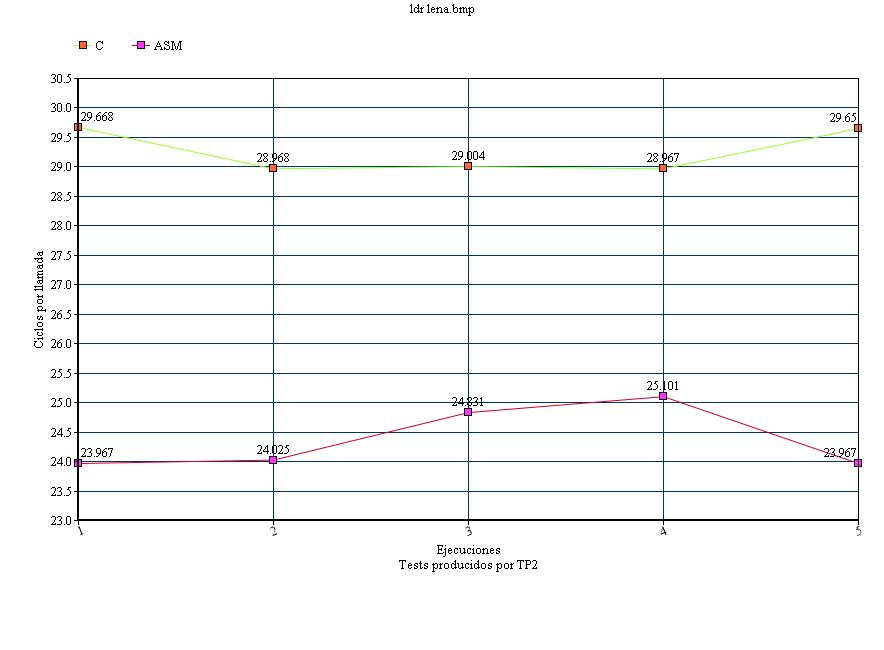
\includegraphics[scale=0.66]{imagenes/ldr-lena-203.jpg}
	\caption{lena-203x203}
	\label{lena-203x203}
  \end{center}
\end{figure}

\newpage
\section{Conclusiones y trabajo futuro}
asdf4


\end{document}

